\documentclass[]{article}

% Imported Packages
%------------------------------------------------------------------------------
\usepackage{amssymb}
\usepackage{amstext}
\usepackage{amsthm}
\usepackage{amsmath}
\usepackage{enumerate}
\usepackage{fancyhdr}
\usepackage[margin=1in]{geometry}
\usepackage{graphicx}
\usepackage{extarrows}
\usepackage{setspace}
%------------------------------------------------------------------------------

% Header and Footer
%------------------------------------------------------------------------------
\pagestyle{plain}  
\renewcommand\headrulewidth{0.4pt}                                      
\renewcommand\footrulewidth{0.4pt}                                    
%------------------------------------------------------------------------------

% Title Details
%------------------------------------------------------------------------------
\title{IdentiSky Detailed Design Document}
\author{Group 2 for SFWR ENG 3A04 \\
\\ 
Alex Guerrero, guerreap, 1133763 \\
Jabrayil Malikov, malikoj, 1302641 \\
Matt Franceschini, francemj, 1310437 \\
Sam Hamel, hamels2, 1321692 \\
Vicky Bilbily, bilbilv, 1317465 \\
}
\date{March 28th, 2016}                                
%------------------------------------------------------------------------------

% Document
%------------------------------------------------------------------------------
\begin{document}

\maketitle	

\section{Introduction}
\label{sec:introduction}
% Begin Section


\subsection{Purpose}
\label{sub:purpose}
% Begin SubSection
\begin{enumerate}[a)]
	\item The purpose of this documents is to show the full design of the system and how it will be implemented.
	\item This document is to be used as a reference for the development team as well as the professor and teaching assistants of SFWR ENG 3A03.4

\end{enumerate}
% End SubSection

\subsection{System Description}
\label{sub:system_description}
% Begin SubSection
\begin{enumerate}[a)]
	\item IdentiSky is a mobile application that identifies objects in the night sky. These objects are limited to constellations and their associated stars, planets, planes, and noteable satellites. Search results are based on the user's current location, date, time, and the user's answers to questions queried by the application. 

\end{enumerate}
% End SubSection

\subsection{Overview}
\label{sub:overview}
% Begin SubSection
\begin{enumerate}[a)]

	\item Included in this document will be diagrams which illustrate how the project will be implemented in code. It also shows all of the use case sequence diagrams, to demonstrate what occurs in each case

	\item The first section will provide an brief overview of the entire document. Section 2 will provide a state chart for each of the application's controller. The next section(section 3) will have a sequence diagram for each use case outlined in the architectural design. In section 4, will be a class diagram which outlines in full detail how each class will be implemented.
	
\end{enumerate}
% End SubSection

% End Section

\section{State Charts for Controller Classes}
\label{sec:state_charts_for_controller_classes}

\begin{figure}[!h]
    \caption{State Chart for Expert Controller class.}
    \centering
    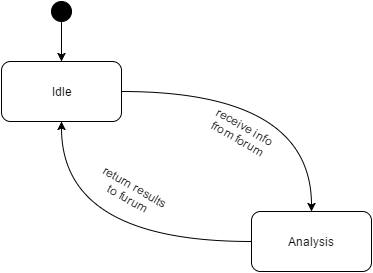
\includegraphics[scale=0.5]{expertcontroller.jpg}
\end{figure}

\begin{figure}[!h]
    \caption{State Chart for Forum class.}
    \centering
    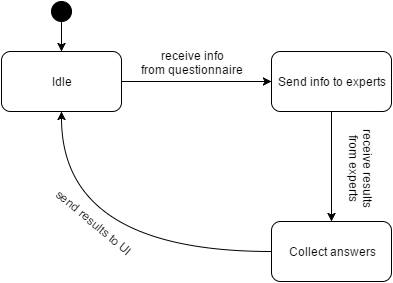
\includegraphics[scale=0.5]{forum.jpg}
\end{figure}

\begin{figure}[!h]
    \caption{State Charts for UI controller class.}
    \centering
    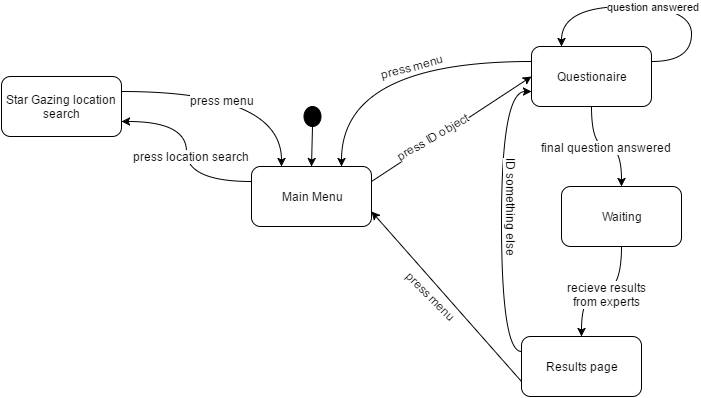
\includegraphics[scale=0.5]{uicontroller.jpg}
\end{figure}

\section{Sequence Diagrams}
\label{sec:sequence_diagrams}
% Begin Section

\begin{figure}[!h]
    \caption{Sequence Diagram for "Identify Object" use case.}
    \centering
    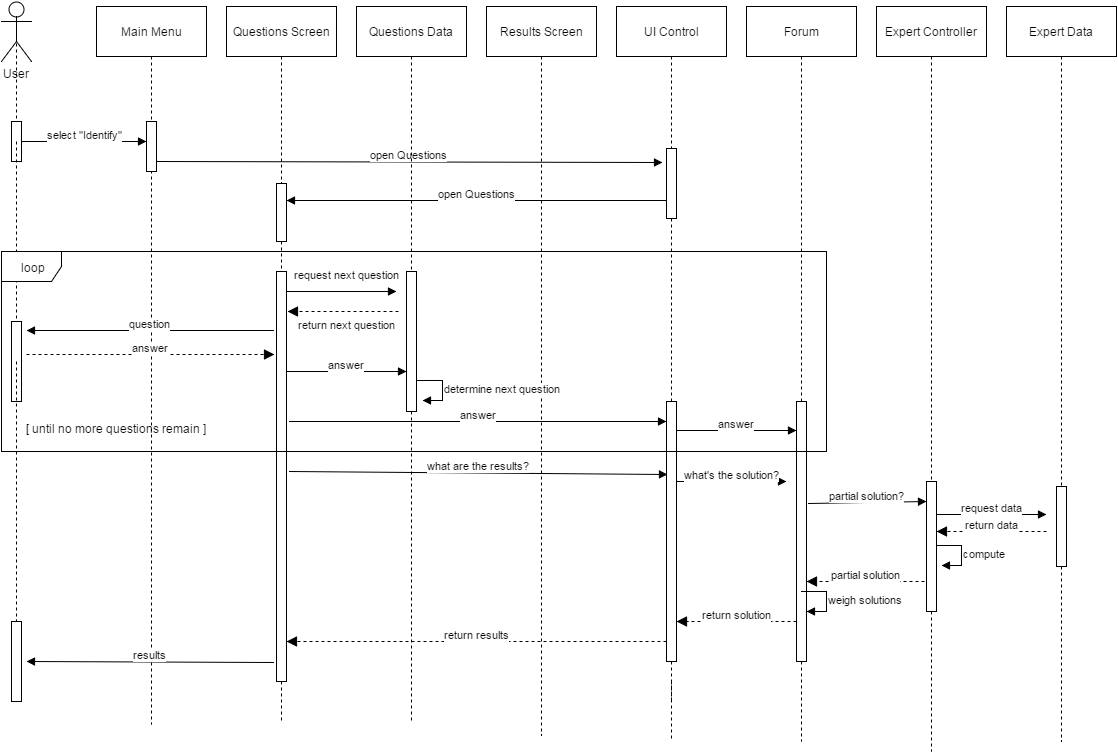
\includegraphics[scale=0.35]{identifyobject.jpg}
\end{figure}

\begin{figure}[!h]
    \caption{Sequence Diagram for "Star-gazing Locations" use case.}
    \centering
    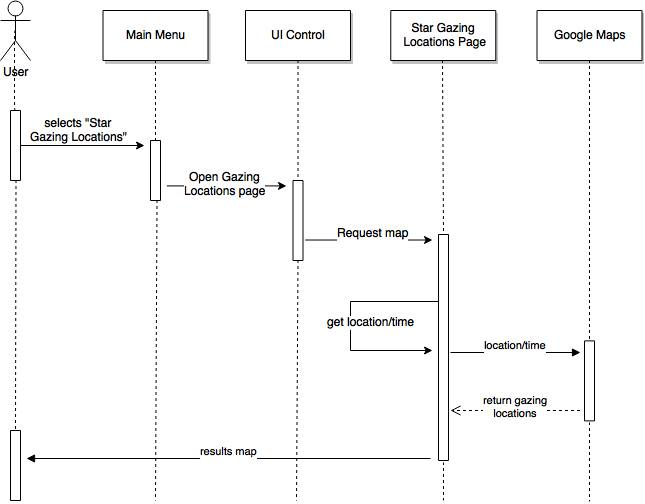
\includegraphics[scale=0.5]{stargazinglocation.jpg}
\end{figure}

\begin{figure}[!h]
    \caption{Sequence Diagram for "View Results" use case.}
    \centering
    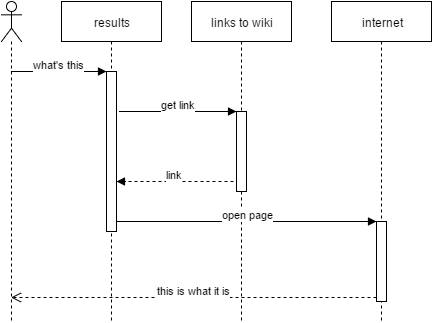
\includegraphics[scale=0.5]{viewresults.jpg}
\end{figure}

% End Section

\section{Detailed Class Diagram}
\label{sec:detailed_class_diagram}
% Begin Section

\begin{figure}[!h]
    \caption{Detailed Class Diagram.}
    \centering
    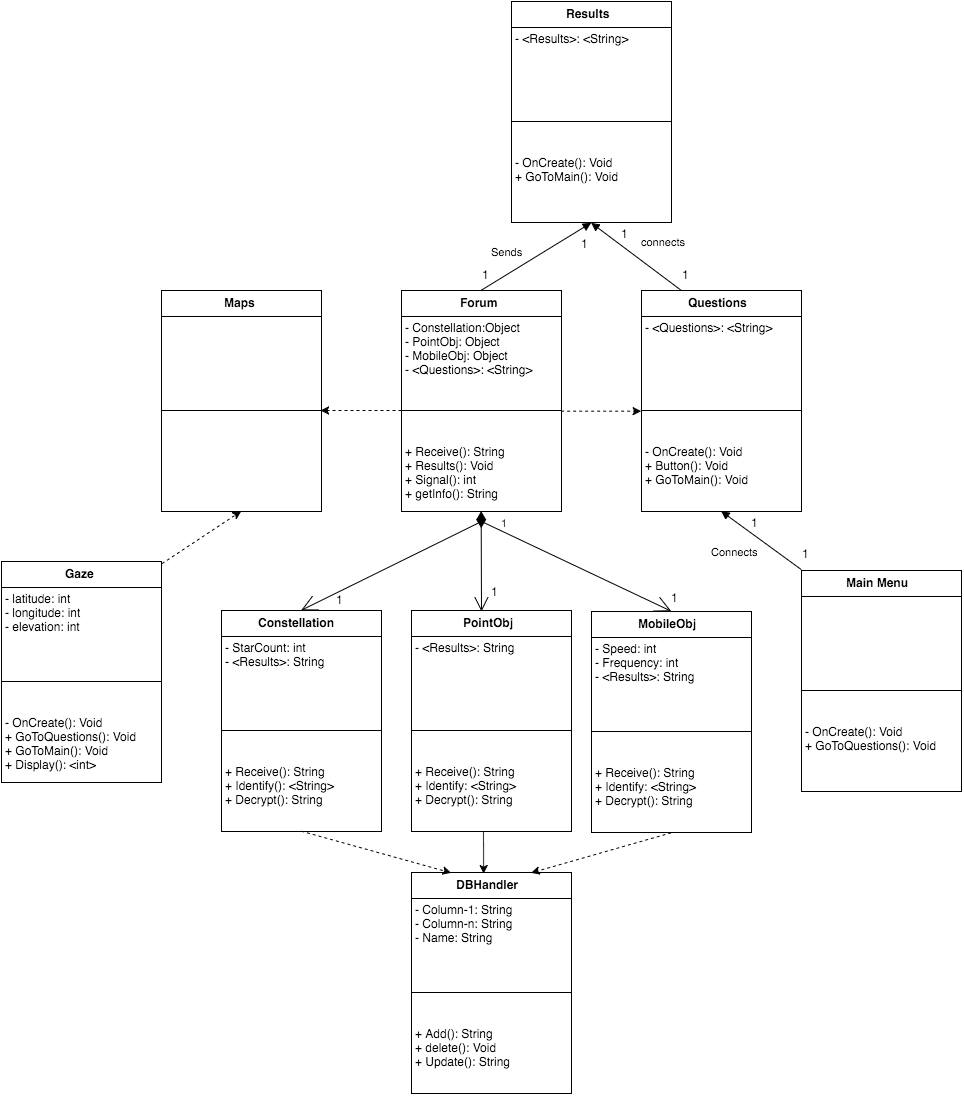
\includegraphics[scale=0.5]{detailedclass.jpg}
\end{figure}

% End Section

\appendix
\section{Division of Labour}
\label{sec:division_of_labour}
% Begin Section
Include a Division of Labour sheet which indicates the contributions of each team member. This sheet must be signed by all team members.
% End Section

\newpage
\section*{IMPORTANT NOTES}
\begin{itemize}
	\item You do \underline{NOT} need to provide a text explanation of each diagram; the diagram should speak for itself
	\item Please document any non-standard notations that you may have used
	\begin{itemize}
		\item \emph{Rule of Thumb}: if you feel there is any doubt surrounding the meaning of your notations, document them
	\end{itemize}
	\item Some diagrams may be difficult to fit into one page
	\begin{itemize}
		\item It is OK if the text is small but please ensure that it is readable when printed
		\item If you need to break a diagram onto multiple pages, please adopt a system of doing so and throughly explain how it can be reconnected from one page to the next; if you are unsure about this, please ask me
	\end{itemize}
	\item Please submit the latest version of Deliverable 1 and Deliverable 2 with Deliverable 3
	\begin{itemize}
		\item They do not have to be a freshly printed versions; the latest marked versions are OK
	\end{itemize}
	\item If you do \underline{NOT} have a Division of Labour sheet, your deliverable will \underline{NOT} be marked
\end{itemize}


\end{document}
%------------------------------------------------------------------------------